% Polycopie pour les etudiants

%\documentclass[handout]{beamer}[10pt, usepdftitle=false]
%\usepackage[printwatermark]{xwatermark}
%\usepackage{pgfpages}
%\pgfpagesuselayout{6 on 1}[a4paper,border shrink=5mm] % 4 par 4

% NE PAS OUBLIER DE BAISSER A QUALITE DU POLYCOPIE!: gs -sDEVICE=pdfwrite -dCompatibilityLevel=1.4 -dPDFSETTINGS=/ebook -dNOPAUSE -dQUIET -dBATCH -sOutputFile=small.pdf big.pdf

% Mes slides pour le cours
\documentclass{beamer}[10pt, usepdftitle=false handout]

\beamertemplatenavigationsymbolsempty

\usepackage[T1]{fontenc}
\usepackage[]{algorithm2e}
\usepackage{multimedia}
\usepackage{gensymb}
\usepackage{textcomp}
\usepackage{array}
\usepackage{fancyvrb}
\usepackage{tabularx,colortbl}

\usepackage{listings}

%\usepackage{background}
%\backgroundsetup{
%    placement=center,
%    scale=5,
%    color=lightgray,
%    contents={PAUL BLONDEL},
%    opacity=0.4
%}
%\setbeamertemplate{background}{\BgMaterial}


%\usepackage[font=small,labelfont=bf]{caption} 

\usetheme{Boadilla}

\title{Introducton to Data Engineering 10}
\author[]{Paul Blondel}
\institute[]{UTSEUS, Shanghai}
\date[]{June 1st, 2021}

\usepackage[style=british]{csquotes}


\def\signed #1{{\leavevmode\unskip\nobreak\hfil\penalty50\hskip1em
  \hbox{}\nobreak\hfill #1%
  \parfillskip=0pt \finalhyphendemerits=0 \endgraf}}

\newsavebox\mybox
\newenvironment{aquote}[1]
  {\savebox\mybox{#1}\begin{quote}\openautoquote\hspace*{-.7ex}}
  {\unskip\closeautoquote\vspace*{1mm}\signed{\usebox\mybox}\end{quote}}


\setbeamertemplate{headline}
{
  \leavevmode%
  \hbox{%
  \begin{beamercolorbox}[wd=1.0\paperwidth,ht=2.25ex,dp=1ex,center]{author in head/foot}%
    \usebeamerfont{author in head/foot}\insertsubsection
  \end{beamercolorbox}}%
  \vskip0pt%
}


\setbeamertemplate{footline}
{
  \leavevmode%
  \hbox{%
  \begin{beamercolorbox}[wd=.5\paperwidth,ht=2.25ex,dp=1ex,center]{author in head/foot}%
    \usebeamerfont{author in head/foot}\insertsection
  \end{beamercolorbox}%
  \begin{beamercolorbox}[wd=.5\paperwidth,ht=2.25ex,dp=1ex,center]{title in head/foot}%
    \usebeamerfont{title in head/foot} \inserttitle \hspace*{2em}  \insertframenumber{} / \inserttotalframenumber\hspace*{2ex} 
  \end{beamercolorbox}}%
  \vskip0pt%
}

\AtBeginSection[]
{
   \begin{frame}
    \tableofcontents[ 
    currentsection] 
   \end{frame}
}

\begin{document}
	{
	\setbeamertemplate{footline}{
  	\leavevmode%
  	\hbox{%
  	\begin{beamercolorbox}[wd=.5\paperwidth,ht=2.25ex,dp=1ex,center]{author in head/foot}%
  	\end{beamercolorbox}%
  	\begin{beamercolorbox}[wd=.5\paperwidth,ht=2.25ex,dp=1ex,center]{title in head/foot}%
  	\end{beamercolorbox}}%
  	\vskip0pt%	
	} 
	\begin{frame}
	\titlepage
	\end{frame}

%	\begin{frame}
%	
%	\begin{aquote}{Dev Ittycheria, President and CEO of MongoDB}
%The cost of managing traditional databases is high. Mistakes made during routine maintenance are responsible for 80 percent of application downtime.
%	\end{aquote}	
%	\end{frame}

	\begin{frame}
		\tableofcontents
	\end{frame}
	}

	\addtocounter{framenumber}{-2}

	\section{Recall}	

    \begin{frame}[label=(first)]
    
	We have seen together how to \textbf{store}, \textbf{manage} and \textbf{process} data...
	\vspace*{0.6em}
	
	Today, we will see how to make your data available to others, we will see:
	\vspace*{0.6em}
	
	\begin{itemize}
	\item{How to \textbf{make your own API} to share data with flask}
	\item{How to \textbf{make an application} with streamlit}
	\end{itemize}		
	
	\end{frame}

	\section{API}
	%\subsection{What is an API?}

	\begin{frame}
	
	\begin{block}{What is an API?}
	An API is a \textbf{set of definitions and protocols facilitating the creation and integration of software applications}. \\ 
	API = "\textbf{Application Programming Interface}"
	\end{block}
	\vspace*{0.6em}

	APIs...
	\vspace*{0.6em}
	
	\begin{itemize}
	\item{allow your product or service to \textbf{communicate with other products and services without knowing implementation details}}
	\item{allow to \textbf{save time and money} (simplify development)}
	\item{give \textbf{flexibility}, \textbf{simplify design}, \textbf{administration}, and \textbf{empower} API users to innovate}
	\item{are perfect to \textbf{make available your data} in a controlled and safe way}
	\end{itemize}
	
	\end{frame}
	
	\begin{frame}
	
Users \textbf{do not need to worry about how to query the database and knowing the business logic} to transforming the data, they just need to know how to call the API to get the data:
\vspace*{0.6em}

	\begin{figure}
	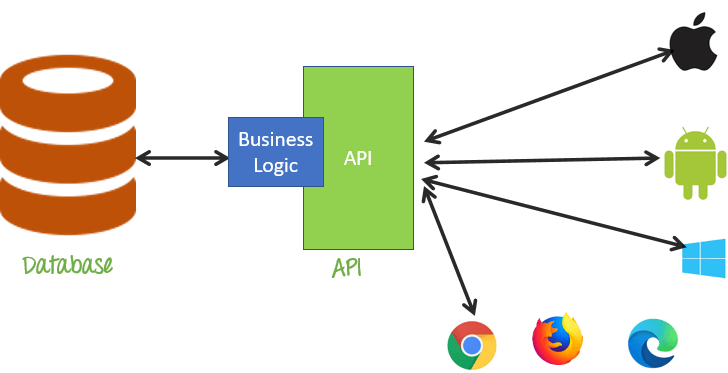
\includegraphics[scale=1.4]{images/api-business-logic.png} 
	\end{figure}

	\end{frame}	
	
	\begin{frame}
	
	There are mainly \textbf{four main types of APIs}: 
	\vspace*{0.6em}

	\begin{itemize}
	\item{\textbf{Open APIs}: \textbf{Publicly available} APIs, there are o restriction to use them (called Public APIs)}
	\item{\textbf{Partner APIs}: Specific rights or licenses permit to access this type of API, they are \textbf{not available to the public}}
	\item{\textbf{Internal APIs}: Internal or private APIs developed by companies to use in their internal systems, to \textbf{enhance work productivity and reduce dependency between software}}	
	\end{itemize}
 
    \end{frame}	
	
		
	\begin{frame}

	When dealing with APIs you will frequently see these terms: 
\vspace*{0.6em}

	\begin{itemize}
	\item{\textbf{HTTP (Hypertext Transfer Protocol):} Protocol permitting communicating data on the web. It implements a number of methods (two most common: GET and POST to push new data to a server}
	\item{\textbf{URL (Uniform Resource Locator):} An address for a resource on the web. A URL consists of a protocol (http://), a domain (website.com), and optional path (/about). A URL describes the location of a specific resource, such as a web page}
	\item{\textbf{JSON (JavaScript Object Notation):} A text-based data storage format that is \textbf{designed to be easy to read for both humans and machines}. JSON is generally the most common format for returning data through an API, XML being the second most common}
	\item{\textbf{REST (REpresentational State Transfer):} A philosophy that \textbf{describes some best practices for implementing APIs}. APIs designed with some or all of these principles in mind are called REST APIs}	
	\end{itemize}

	\end{frame}
	
	\begin{frame}
	
	\underline{\textbf{The book distributor example:}}
	\vspace*{0.6em}	
	
	\begin{itemize}
	\item{\underline{But:} Distributor may want to provide an application to check the availability of the books}	
	\item{\underline{Remark:} making an application might be expensive and time-consuming (and require ongoing maintenance)}
	\item{\underline{Alternatively:} \textbf{the distributor can just provide an API} to check inventory availability}
	\end{itemize}		
	
	Opting for an API in this case has numerous advantages:
\vspace*{0.6em}

\begin{enumerate}
\item{Customers have the \textbf{ability to centralize their inventory} information by accessing the API}
\item{Distributor can change the internal system of the API and \textbf{not impact the customer experience}}
\item{It is \textbf{easy for others to develop applications plugged to it}, easy to spread data to other systems}
\end{enumerate}

	\end{frame}	

\begin{frame}
In this course we are interested in \textbf{remote APIs}:
\vspace*{0.6em}

\begin{itemize}
\item{Remote APIs: designed to \textbf{interact via a communication network}}
\item{Resources manipulated by the \textbf{API are not located on the computer making the request}}
\item{Most remote APIs are designed \textbf{based on Web standards}}
\item{Not all remote APIs are Web APIs, but it can be assumed that all Web APIs are remote}
\item{Web APIs typically use the \textbf{HTTP protocol}}
\item{Response messages are most often in the form of \textbf{XML} or \textbf{JSON}}
\end{itemize}

\end{frame}	

\begin{frame}

There are two main way to build remote APIs:
\vspace*{0.6em}

\begin{itemize}
	\item{\textbf{SOAP (Simple Objects Access Protocol):} 
		\begin{itemize}
			\item{APIs designed according to the SOAP protocol use the XML format for their messages and receive requests via HTTP or SMTP}
			\item{SOAP aims to simplify the exchange of information between applications that run in different environments or that were written in different languages}
		\end{itemize}	
		}	 
	\item{\textbf{REST (Representational State Transfer)\
	
	{In this course we will only talk about this type of API}:} 
		\begin{itemize}
			\item{Another attempt of API standardization}
			\item{Web APIs meeting all the constraints of the REST architecture are called RESTful APIs}
			\item{REST is an architectural style (contrary to SOAP, which is a protocol)}
		\end{itemize}			}
\end{itemize}

\end{frame}
	
\section{REST API}

\begin{frame}

List of principles of a RESTful API:
\vspace*{0.6em}

\begin{enumerate}
\item{\textbf{Client-server}: Composed of clients servers, and resources and it processes requests via the HTTP protocol}
\item{\textbf{Stateless}: Client content is never stored on the server between requests (session state information is stored on the client)}
\item{\textbf{Cacheable}: Caching brings performance improvement for the client-side and reduce the load}
\item{\textbf{Layered system}: Additional layers can perform additional functions: load balancing, cache sharing or security}
\item{\textbf{Code on demand (optional)}: Can extend the functionality of a client by returning executable code (permitted)}
\item{\textbf{Uniform interface}: Resources should be accessible through a \textbf{common approach} and modified using a \textbf{consistent approach}}
\end{enumerate}

\begin{block}{REST or RESTFUL?}
RESTful services means it \textbf{follows all the above principles} \\
REST based services \textbf{follow some of the above principles and not all}
\end{block}

\end{frame}

\begin{frame}

\begin{itemize}
\item{REST APIs permit all possible \textbf{CRUD} operations:
	\begin{itemize}
		\item{\textbf{C}reate}
		\item{\textbf{R}etrieve}
		\item{\textbf{U}pdate}
		\item{\textbf{D}elete}
	\end{itemize} }
\item{REST guidelines suggest...
	\begin{itemize}
		\item{...\textbf{a specific HTTP method}}
		\item{...for \textbf{a particular type of API call}}
	\end{itemize} 
	}
	\item{Technically possible to violate the guidelines, but \textbf{highly discouraged}}
\end{itemize}

\end{frame}

\begin{frame}
What is \textbf{HTTP}?
\vspace*{0.6em}

\begin{columns}[c]
\column{.5\textwidth}
\begin{itemize}
	\item{HTTP is a protocol allowing the \textbf{fetching of resources}, such as HTML documents}
	\item{At the foundation of any data exchange on the Web, it's a \textbf{client-server protocol}}
	\item{Requests are \textbf{initiated by the recipient}, usually the Web browser}
	\item{Full document \textbf{rebuilt from different sub-documents} (text, images, videos, etc.)}

\end{itemize}

\column{.5\textwidth}
\begin{figure}
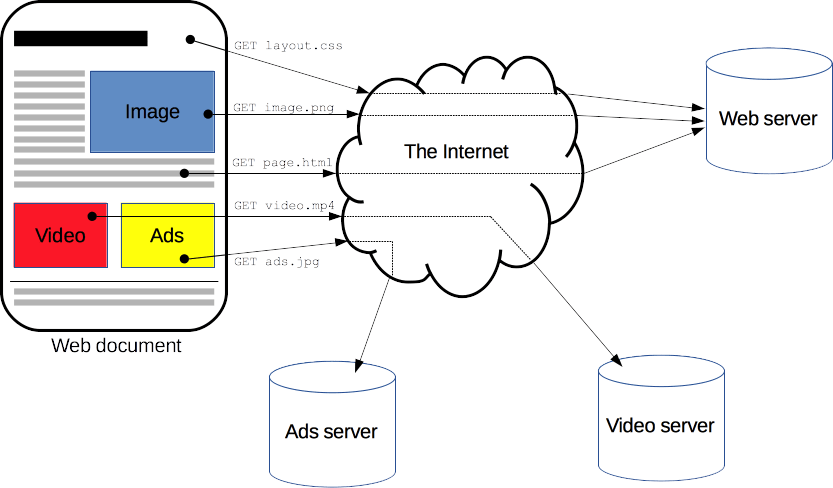
\includegraphics[scale=0.8]{images/http-diagram.png} 
\end{figure}

\end{columns}

%\begin{block}{WWW} 
%World Wide Web is about communication between web clients and web servers. Clients are often browsers (Chrome, Edge, Safari), but they %can be any type of program or device. Servers are most often computers in the cloud.
%\end{block}
\end{frame}

\begin{frame}

How \textbf{HTTP Communication between clients and servers} is handled:
\vspace*{0.6em}

\begin{itemize}
\item{A client sends a HTTP request to the web}
\item{A web server receives the request}
\item{The server runs an application to process the request}
\item{The server returns an HTTP response (output) to the browser}
\item{The client (the browser) receives the response}
\end{itemize}
  
\begin{block}{HTTP and REST APIs}
REST APIs use HTTP protocol to transmit requests and get results \underline{but}:
\begin{itemize}
\item{not necessarily through the Web}
\item{not necessarily from a Web browser}
\end{itemize}
\end{block}


\end{frame}

\begin{frame}

%multicolums ici

A request to fetch content from a server contains:
\vspace*{0.6em}

\begin{columns}[c]
\column{.5\textwidth}

\begin{itemize}
\item{A \textbf{Path} to requested web page}
\item{A \textbf{Protocol Version}}
\item{A \textbf{Method} (GET, POST, other)}
\item{\textbf{Headers} containing info about the client}
\item{(Eventually) A \textbf{Body} containing data to send}
\end{itemize}

\column{.5\textwidth}

\begin{figure}
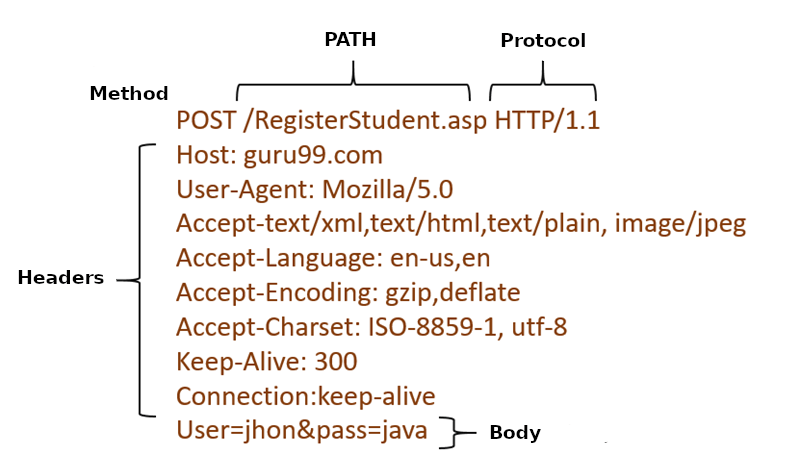
\includegraphics[scale=0.2]{images/http.png} 
\end{figure}

\end{columns}

\end{frame}

\begin{frame}

\begin{columns}[c]
\column{.5\textwidth}
The response:
\vspace*{0.6em}

When the server responds, it returns a \textbf{requested content}, or a \textbf{result}, plus a \textbf{code}. \\
(404 error code: content not found) 


\column{.5\textwidth}
There are many others code:
\vspace*{0.6em}
\begin{itemize}
\item{Code 500: an error occurred on the server}
\item{Code 401: access to this web page is not allowed}
\item{Code 400: client's request is badly formed}
\item{Code 200: everything went well}
\item{...}
\end{itemize}
\end{columns}

	\begin{figure}
	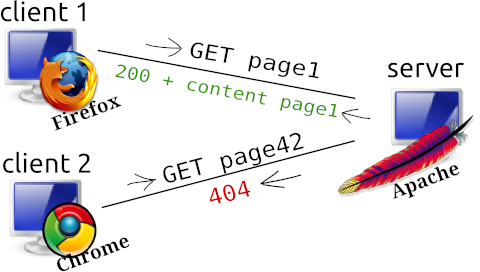
\includegraphics[scale=1.2]{images/http-codes-example.png} 
	\end{figure}




\end{frame}

\begin{frame}


\begin{center}
\begin{tabular}{m{2cm}|m{2cm}|m{3cm}|m{3cm}}
\textbf{HTTP Method} & \textbf{CRUD} & \textbf{Entire Collection (e.g. /users)} & \textbf{Specific Item (e.g. /users/123)} \\ \hline
\textbf{POST} & Create & 201 (Created) & Avoid using POST on single resource \\ \hline
\textbf{GET} & Read & 200 (OK) + list of users & 200 (OK) + a user or 404 (Not Found)  \\ \hline
\textbf{PUT} & Update \newline Replace & 405 (Should not be allowed) & 200 (OK), 204 (No Content) or 404 (Not Found) \\ \hline
\textbf{PATCH} & Partial \newline Update & 405 (Should not be allowed) & 200 (OK), 204 (No Content) or 404 (Not Found) \\ \hline 
\textbf{DELETE} & Delete & 405 (Should not be allowed) & 200 (OK) or 404 (Not Found) \\ \hline
\end{tabular}
\end{center}

\end{frame}

\section{Flask}

\begin{frame}

What is Flask?
\vspace*{0.6em}

	\begin{figure}
	
\includegraphics[scale=1.4]{images/flask.png} 
	\end{figure}

\begin{itemize}
\item{Flask is a \textbf{web framework} for Python
	\begin{itemize}
		\item{it provides functionality for \textbf{building web applications}}
		\item{it can \textbf{manage HTTP requests} and \textbf{render templates}}
	\end{itemize} }
\item{Flask is easy: it can \textbf{save time and effort} for programmers}
\item{One can easily build a HTTP REST/RESTful API with it}
\end{itemize}

\end{frame}

\begin{frame}
Let's analyze this address before starting: "http://www.siteduzero.com/forum-81-407-langage-python.html"
\vspace*{0.6em}

\begin{itemize}
\item{"http" is the \textbf{protocol}}
\item{"www.siteduzero.com": is the \textbf{domain name}}
\item{"/forum-81-407-language-python.html": is the path to the requested content (also called \textbf{route})}
\item{The full address is often called a "\textbf{endpoint}"}
\end{itemize}
\vspace*{0.6em}

In this course the HTTP server will be hosted on our own computer:
\vspace*{0.6em}

\begin{itemize}
\item{The "domain name" of our own computer is called "\textbf{localhost}" by convention}
\item{With Flask, the default port is 5000}
\item{The route "hello" is thus accessible through the URL: "http://loclahost/hello"}
\end{itemize}

\end{frame}
\begin{frame}[fragile]

Let's begin with a simple code example (we will name our file "hello.py"):
\vspace*{0.6em}

\begin{verbatim}
from flask import Flask
app = Flask(__name_)

@app.route('/hello/', methods=['GET', 'POST'])
def welcome():
    return "Hello World!"

if __name__ == '__main__' :
app.run()
\end{verbatim}

\begin{enumerate}
\item{Execute the code by simply typing: "\textbf{python hello.py}" in the terminal}
\item{You should see something like this:
\begin{verbatim}
* Running on http://localhost:5000/ (Press CTRL+C to quit)
\end{verbatim}}
\item{Then open your web browser and go to \textbf{http://localhost:5000/hello/}}
\item{You should see a "Hello World!" appearing...}
\end{enumerate}
	

\end{frame}
\begin{frame}[fragile]
Let's analysis this code line-by-line:
\vspace*{0.6em}

\begin{itemize}
\item{\textbf{from flask import Flask} → Import the Flask class}
\item{\textbf{app = Flask(\_\_name\_\_)} → Create an instance of the class}
\item{\textbf{@app.route('/hello/', methods=['GET', 'POST'])} → the route() decorator tell Flask what URL should trigger the function 
and the HTTP methods that are allowed (default is ['GET'])}
\item{\textbf{if \_\_name\_\_ == '\_\_main\_\_':} → This line ensures that our Flask app runs only when it is executed as the main file and not when imported in some other file}
\item{\textbf{app.run()} → Run the Flask application
host specifies the server on which we want our flask application to run (default host value is localhost or 127.0.0.1)}
\end{itemize}

\end{frame}
\begin{frame}[fragile]
Adding a route is easy using the following Python decorator before a function definition:
\vspace*{0.6em}

\begin{verbatim}
@app.route('/ROUTENAME/', methods=['GET’])
def my_function :
    ...
    return ...
end
\end{verbatim}
\vspace*{0.6em}

\end{frame}
\begin{frame}[fragile]
JSON serializable output:
\vspace*{0.6em}

\begin{itemize}
\item{The return value of a function in a Flask app should be a JSON object}
\item{You can use \textbf{jsonify} to make your output a JSON
	\begin{itemize}
		\item{This returns a JSON output as a "\textbf{Response object}" with \textbf{application/json mime-type}}
	\end{itemize}
}
\end{itemize}
\vspace*{0.6em}

Example:
\vspace*{0.6em}

\begin{verbatim}
from flask import jsonify
@app.route('/person/')
def hello():
    return jsonify({'name':'Jimit',
                    'address':'India'})
This will send a JSON response like this:
{
  "address": "India", 
  "name": "Jimit"
}
\end{verbatim}


\end{frame}
\begin{frame}
\textbf{Example of a RESTful API:}
\vspace*{0.6em}

\underline{\textbf{Goal:}} An API to get book(s), add (a) book(s), update book(s) and remove (a) book(s) from a DB
\vspace*{0.6em}

We must have two routes:
\vspace*{0.6em}

\begin{itemize}
\item{\textbf{/books}: to perform action on book collection: list books, add a book, etc}
\item{\textbf{/books/id}: to perform action on a book item: show, update or delete}
\end{itemize}

\begin{block}{References}
A similar example here: 
\begin{itemize}
\item{https://www.kite.com/blog/python/flask-restful-api-tutorial/}
\end{itemize}
Official documentation for Flask 1.1: 
\begin{itemize}
\item{https://flask.palletsprojects.com/en/1.1.x/}
\end{itemize}
\end{block}

\end{frame}
\begin{frame}[fragile]
\begingroup
\fontsize{6pt}{8pt}\selectfont
\begin{verbatim}
@app.route('/books', methods = ['GET', 'POST'])
def booksFunction():
   if request.method == 'GET':
       return getBooks()
   elif request.method == 'POST':
       title = request.args.get('title', '')
       author = request.args.get('author', '')
       genre = request.args.get('genre', '')
       return makeANewBook(title, author, genre)

@app.route('/books/', methods = ['GET', 'PUT', 'DELETE'])
def bookFunctionId(id):
   if request.method == 'GET':
       return geABook(id)
 
   elif request.method == 'PUT':
       title = request.args.get('title', '')
       author = request.args.get('author', '')
       genre = request.args.get('genre', '')
       return updateABook(id,title, author,genre)
  
   elif request.method == 'DELETE':
       return deleteABook(id)
\end{verbatim} 
\endgroup      
       
\begin{block}{Recall}
getBooks, makeANewBook, getABook, updateABook, deleteABook should \textbf{return a JSON} and a \textbf{HTTP status or code} (200, 404, 500, etc.)
\end{block}       
       
\end{frame}
\begin{frame}[fragile]
Now, how to interrogate our API?
\vspace*{0.6em}

For example, to get all the list of all books we should do the following GET API call with curl:
\vspace*{0.6em}

\begin{verbatim}
$ curl -v http://localhost:5000/books
\end{verbatim}

If you want to add a book to the database through the API and with curl:
\vspace*{0.6em}

\begingroup
\fontsize{6pt}{8pt}\selectfont
\begin{verbatim}
$ curl -d '{"title":’Book’,"author’ :’Jean’,"genre" :’science-fiction’}' 
-H 'Content-Type: application/json' http://localhost:5000/books/
\end{verbatim}
\endgroup

If you want to delete a book:
\vspace*{0.6em}

\begin{verbatim}
$ curl -X DELETE http://localhost:5000/books/9
\end{verbatim}

If you want to get informaiton about a specific book:
\vspace*{0.6em}
\begin{verbatim}
$ curl -v http://localhost:5000/books/9
\end{verbatim}
\end{frame}
\begin{frame}[fragile]
If you want to update the information of a book:
\vspace*{0.6em}
\begingroup
\fontsize{6pt}{8pt}\selectfont
\begin{verbatim}
$ curl -d ‘{"title":’Book’,"author’ :’Jean-Jaques’,"genre" :’science-fiction’}' 
-H 'Content-Type: application/json' -X PUT http://localhost:8082/books/9
\end{verbatim}
\endgroup

Note that we can also call the API using the Python requests module:

\begingroup
\fontsize{6pt}{8pt}\selectfont
\begin{verbatim}
# !/usr/bin/python
import requests
response = requests.get('http://localhost:5000/books/10')
print(response.json())

# Create a new resource
data_1 = {'title':'titre 2', ‘author’ : ‘Patrick’, ‘genre’ : ‘History’}
response = requests.post('http://localhost:5000/books', data = data_1)
print(response.json())

# List of books
response = requests.get('http://localhost:5000/books')
print(response.json())

# Update an existing resource
data_2 = {'title':'Titre 2', ‘author’ : ‘Patrick’, ‘genre’ : ‘History’}
requests.put('http://localhost/books/454', data = data_2)
print(response.json())

response = requests.delete('http://localhost:5000/books/10')
print(response.json())
\end{verbatim}
\endgroup

\end{frame}
\section{Streamlit}

\begin{frame}


\begin{columns}[c]
\column{.5\textwidth}

What is Steamlit ?
\vspace*{0.6em}

\begin{itemize}
\item{The "\textbf{fastest way to build and share data apps}"}
\item{Works with \textbf{Python} (plain Python code)}
\item{Extremely \textbf{easy}}
\item{Streamlit data apps can be created just by using the \textbf{streamlit module}}
\item{Run your app in your terminal like a Python script: \textbf{streamlit run script\_name.py}}
\end{itemize}

\column{.5\textwidth}

\begin{figure}
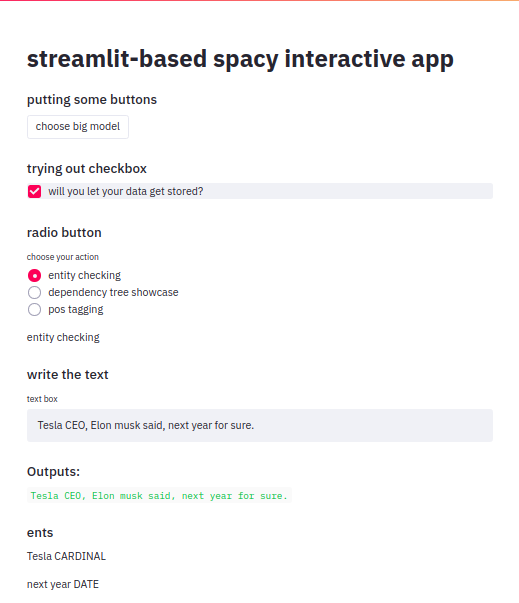
\includegraphics[scale=1.2]{images/streamlit.png} 
\end{figure}	

\end{columns}

\end{frame}

\begin{frame}
Streamlit support different representations (seaborn, matplot, etc) and much can be written using the following functions:
\vspace*{0.6em}

\begin{itemize}
\item{\textbf{st.title()}: 
Create a title element in the data app (useful method to give a proper heading to your app)}
\item{\textbf{st.write()}:
The "swiss army knife" of streamlit: you can use it to print or show or display elements in your app using this method}
\item{\textbf{st.subheader()}:
Create different sections in an app (create big and bold texts and displays them properly helps creating sections in your app)}
\end{itemize}


\end{frame}
\begin{frame}[fragile]

Example of code:
\vspace*{0.6em}

\begingroup
\fontsize{6pt}{8pt}\selectfont
\begin{verbatim}
import streamlit as st
import numpy as np
import pandas as pd
import altair as alt

st.title("The first basic testing app")
st.write("\frac{1}{2} does it support lateX?")
st.write("looks like it doesn't")
st.write("a normal string")
st.write("<b>food</b> is great here; checking if simple html works", unsafe_allow_html = True)
st.write("thanks, its a *good* day", unsafe_allow_html = True)
st.write("displaying that numbers can be represented")
st.write(1234)
st.write("showing that dataframes can be printed")
st.write(pd.DataFrame({"first_column":[10,20,30,40],"second_column":[105,405,905,1605]}))
st.write("we can show headers also")
st.header("it shows chart too")

\end{verbatim}
\endgroup

\end{frame}
\begin{frame}[fragile]
Rest of the code:
\vspace*{0.6em}

\begingroup
\fontsize{6pt}{8pt}\selectfont
\begin{verbatim}
df = pd.DataFrame(np.random.randn(200, 3),
                  columns=['a', 'b', 'c'])
c = alt.Chart(df).mark_circle().encode(x='a', y='b',size='c',color='c',tooltip=['a', 'b', 'c'])
st.write(c)
st.subheader("showing a codeblock using st.code")
code = """for i in range(20):
           print("this is a count of" + str(i))
       """
st.code(code,language = "python")
df = pd.DataFrame(np.random.randn(20,8),
                  columns = ["columns_"+str(i) for i in range(1,9)])
st.subheader("showing dataframe as table")
st.table(df)
\end{verbatim}
\endgroup

Once you created your python file, run the Streamlit application like this:
\vspace*{0.6em}

\begin{verbatim}
$ streamlit run app.py
\end{verbatim}

And open the application in your browser...

\end{frame}
\begin{frame}[fragile]
It is also possible to add \textbf{checkboxes}, \textbf{radios}, \textbf{text inputs}, \textbf{buttons}, etc. 
\vspace*{0.6em}

\textbf{st.button()}: take a label in input. It return a boolean value, if the button is clicked in the app then it returns True otherwise False.
\vspace*{0.6em}

\begin{verbatim}
if st.button("choose big model"):
    nlp = spacy.load("en_core_web_lg")
else:
    nlp = spacy.load("en_core_web_sm")
\end{verbatim}

\end{frame}
\begin{frame}[fragile]
\textbf{st.checkbox()} is a similar to st.button(), it takes a label and returns a bool return value (but a box is showed in the UI):

\begin{verbatim}
st.subheader("trying out checkbox")
check = st.checkbox("will you let your data get stored?") 
if check:
    print("fake notion! nothing recording now!")
else:
    pass
\end{verbatim}

\end{frame}
\begin{frame}[fragile]
\textbf{st.text\_input()}: returns the text written in the text box... It is a very powerful tool. see below how we implemented it:
\vspace*{0.6em}

\begin{verbatim}
st.subheader("write the text")
text = st.text_input("text box","Example: write here")
\end{verbatim}

\begin{block}{Official documentation}
More information and content in the official Steamlit documentation :
https://docs.streamlit.io/en/stable/
\end{block}
\end{frame}
\end{document}